This section aims to outline the basic design and architecture of the artefact.

\section{System Architecture}
The sentiment analysis tool will be built as a desktop application developed in Python. The system architecture consists of three main elements: the GUI, the chosen machine-learning model for sentiment analysis, and the integration with social media APIs for data retrieval. This section will go into more detail on the specific design and architecture of the application.

\begin{figure}[h]
    \centering
    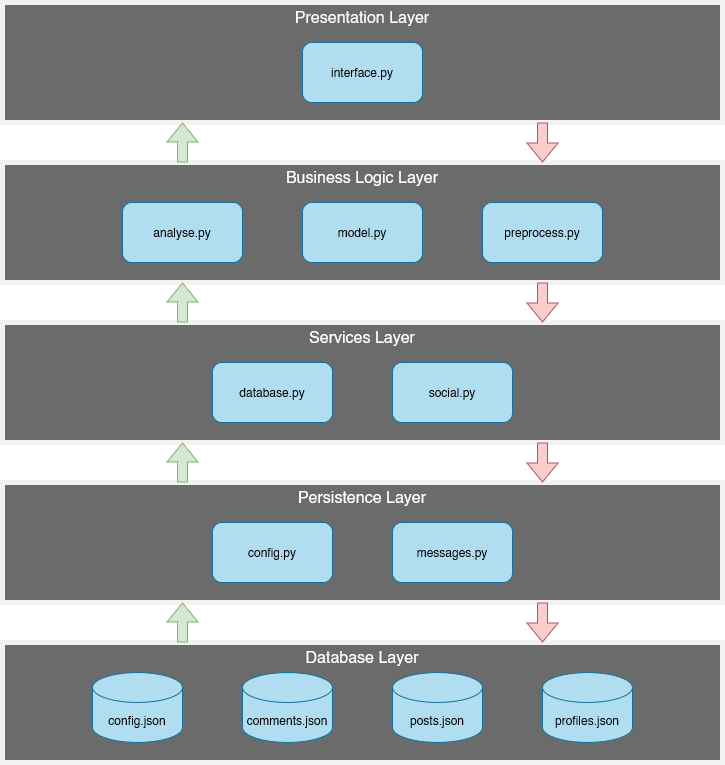
\includegraphics[width=0.8\textwidth]{figures/system-architecture-layers.png}
    \caption{Proposed system layer architecture.}
\end{figure}

    \subsection{Architectural Style}
    The system uses a layered architecture, dividing the application into distinct layers containing components based on their function and responsibility. This style promotes modularity, scalability, and maintainability by separating concerns and enforcing clear boundaries between different parts of the system. The layered architecture also allows for easy integration of new features int he future.

    \subsection{Layers and Components}
    The system comprises of five main layers: presentation layer, business logic layer, services layer, persistence layer, and database layer.

        \subsubsection{Presentation Layer}
        The presentation layer is responsible for presenting the processed and analysed data to the user. In \pinline{interface.py} there will be various classes for building and handling the windows and their layouts; there will also be classes for handling functions on other threads in order to preserve the functionality of the GUI while long running operations are in progress.

        \subsubsection{Business Logic Layer}
        The business logic layer is responsible for interpreting the data provided by the layers below. \pinline{analyse.py} will handle the analysis of data, for example the creation of a line chart which plots the sentiment over a given time frame. \pinline{model.py} will contain a class for the machine-learning model which will handle training of the model as well as making predictions using the model. Finally, \pinline{preprocess.py} will be responsible for processing and cleaning text before training/making predictions.

        \subsubsection{Services Layer}
        The services layer is responsible for interacting with the social media APIs and the data sources. In this layer there is \pinline{database.py}, which collects and manipulates post data from the APIs and any stored, previously collected data. Meanwhile, \pinline{social.py} will contain classes for the social media APIs, with functionality for scraping posts with given search terms.

        \subsubsection{Persistence Layer}
        The persistence layer is responsible for the persistence of configuration, settings, and logging errors and messages. It will consist of two modules: \pinline{config.py} and \pinline{messages.py}, which will have simple functions intended for retrieving data from the database layer and sending messages to the console respectively.

        \subsubsection{Database Layer}
        The database layer is responsible for storing persistent data used by the application. \pinline{config.json} will store all of the configuration settings of the app, while \pinline{profiles.json} will store the specific configurations for each profile in terms of searching social media. Lastly, \pinline{posts.json} and \pinline{comments.json} will store collected posts and comments respectively, with all the necessary information for analysis such as the body text, the amount of favourites, the predicted sentiment, and specific to comments, the parent post (to allow for contextual analysis).

    \subsection{Key Components}
    The key components and their important classes are as follows:
    \begin{itemize}
        \item \pinline{interface.py}: this module will handle everything to do with the GUI.
        \begin{itemize}
            \item \pinline{MainWindow()}: this class will be responsible for building the main window and handling any interactions the user may have with it.
            \item \pinline{SubWindow()}: there will be various classes for handling sub-windows such as profile editor and settings.
            \item \pinline{Worker()}: this will be a class for handling multithreaded long-running tasks to keep the GUI responsive in the meantime.
        \end{itemize}
        \item \pinline{model.py}: the module for handling everything to do with the machine-learning models.
        \begin{itemize}
            \item \pinline{BERTModel()}: this class will handle the training and predicting for a BERT model.
            \item \pinline{LSTMModel()}: the class for handling the training and predicting for a LSTM model
            \item \pinline{PFDualBERTModel()}: this class will handle training and predicting for a PFDualBERT model. 
        \end{itemize}
        \item \pinline{database.py}: this module will handle everything to do with the collection of data from the databases, as well as the merging of this data with new social media posts.
        \begin{itemize}
            \item \pinline{PostCollector()}: a class to collect and merge data from social media with existing stored data.
        \end{itemize}
        \item \pinline{social.py}: the module responsible for scraping social media's posts with given search parameters.
        \begin{itemize}
            \item \pinline{XScraper()}: this class will interface with the X API to collect posts for a given search term.
            \item \pinline{RedditScraper()}: this class will interface with the Reddit API to collect posts from given subreddits with given search parameters.
        \end{itemize}
    \end{itemize}

\section{Data Model}
As the artefact will involve the storage and retrieval of data, it is appropriate to model the relationships between different entities within the data. The data model consists of three entities: profile, post, and comment; each profile will have a number of posts collected for its specified subreddits, and each post will have a number of comments collected with it if this setting is enabled. Both the posts and comments databases will be in a directory labeled with the profile ID.

For this project, it was decided that json format would be acceptable for storing data, this is due to the portable, efficient, and scalable nature of json, along with the lack of a need for anything with more complex functionality. The json data will be read and temporarily stored in a \pinline{pandas.DataFrame} structure while being used by the programme.

\begin{figure}[h]
    \centering
    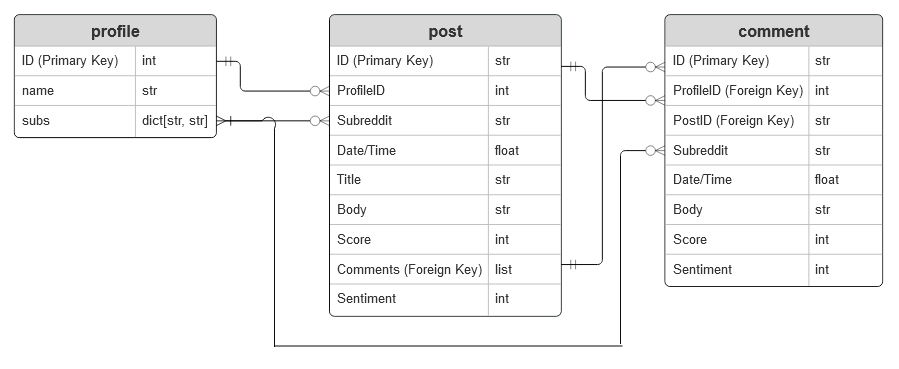
\includegraphics[width=\textwidth]{figures/database-relationship-diagram.png}
    \caption{Relational diagram showing the database structure.}
\end{figure}

\section{Graphical User Interface}
The goal of this interface is to be easily accessible, clearly show the analysis of data, and look visually professional. The interface will consist of three main windows: the main window, where majority of the functionality happens and all the data is displayed, the profile editor window, where the user can add and edit brand profiles, and finally the settings window, where the user can change settings that affect the system functionality and visuals.

The main window will consist of three main areas: the main toolbar at the top of the window containing various buttons, the time-frame selector along with text describing the profile sentiment, and an analysis panel with tabs to visualise the data in various ways.

\begin{figure}[h]
    \centering
    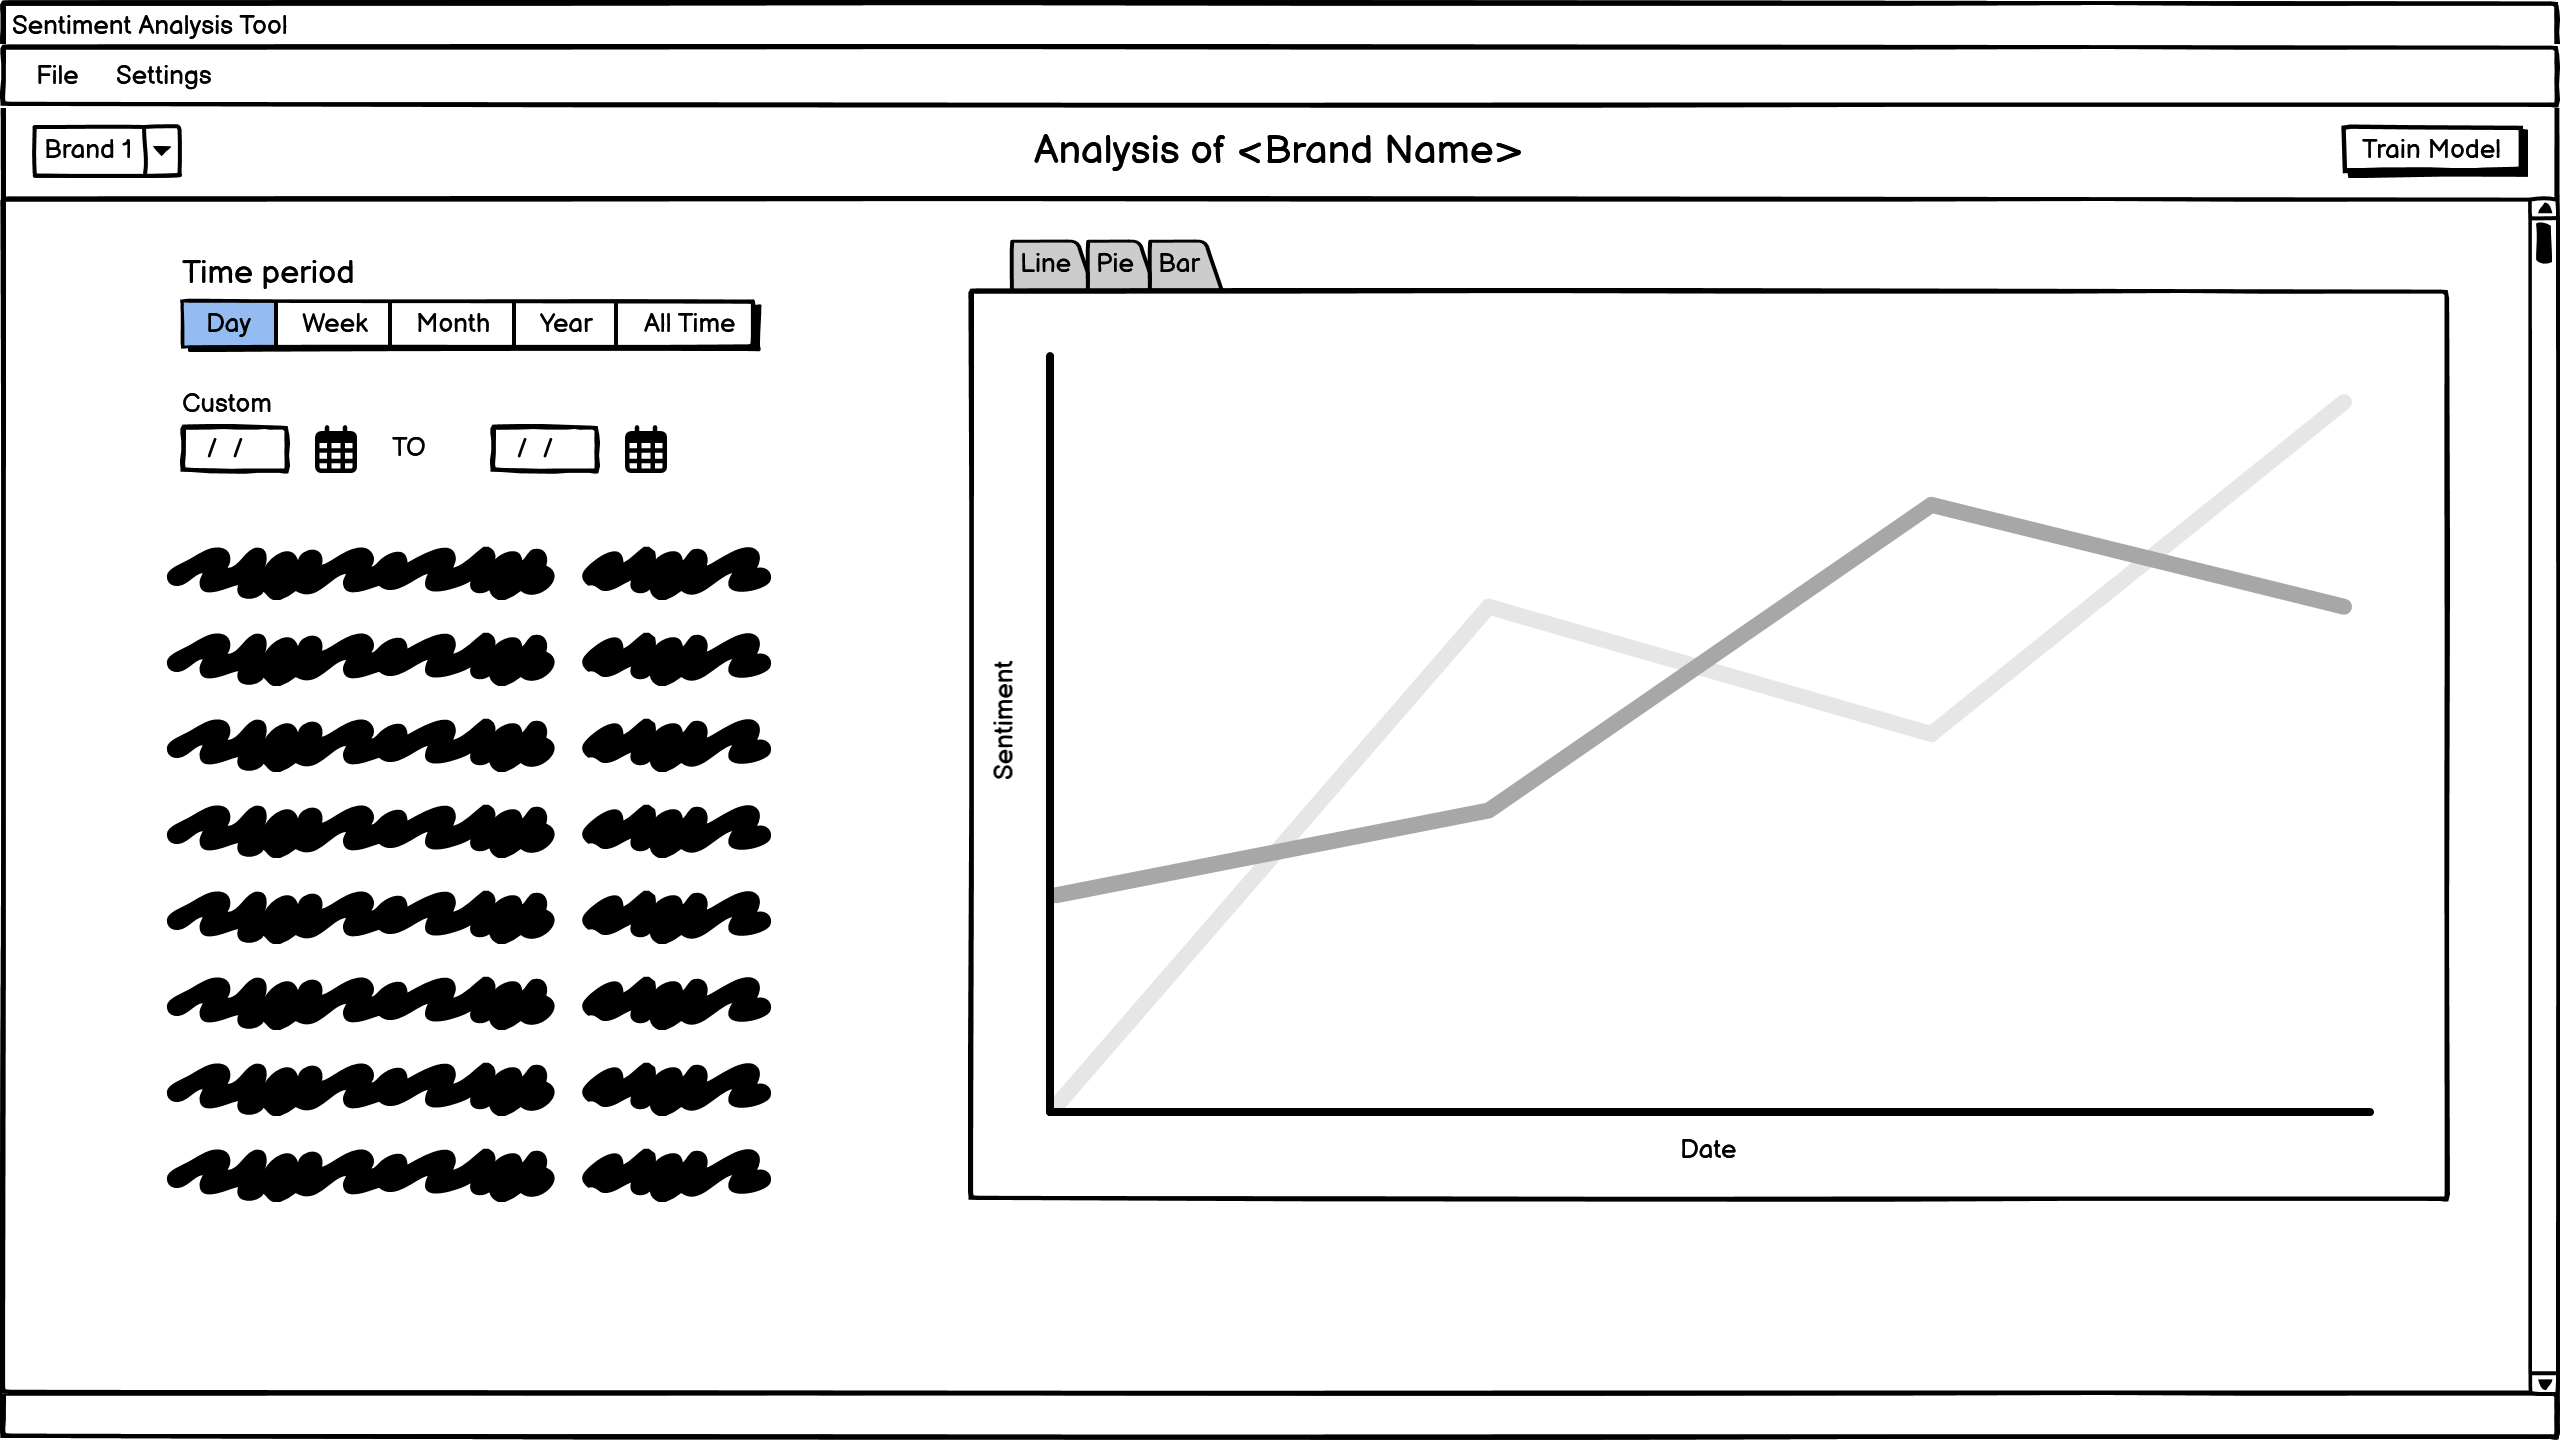
\includegraphics[width=\textwidth]{figures/wireframe-main.png}
    \caption{Wire-frame of the proposed main GUI.}
\end{figure}

The profile editor window must allow the user to easily create and edit profiles, to do this it will have a text bar for choosing the profile name, along with two buttons ``enter'' and ``delete'', which will either save or delete the profile respectively. It must also allow them to add subreddits with search terms to this profile, to do this there will be two text boxes, one for the subreddit name, and one for the terms to search for in that subreddit. When a subreddit is added to the profile, it will appear in a row below these text boxes, here the user can click the ``remove'' button to remove a subreddit and its search terms from the profile.

\begin{figure}[h]
    \centering
    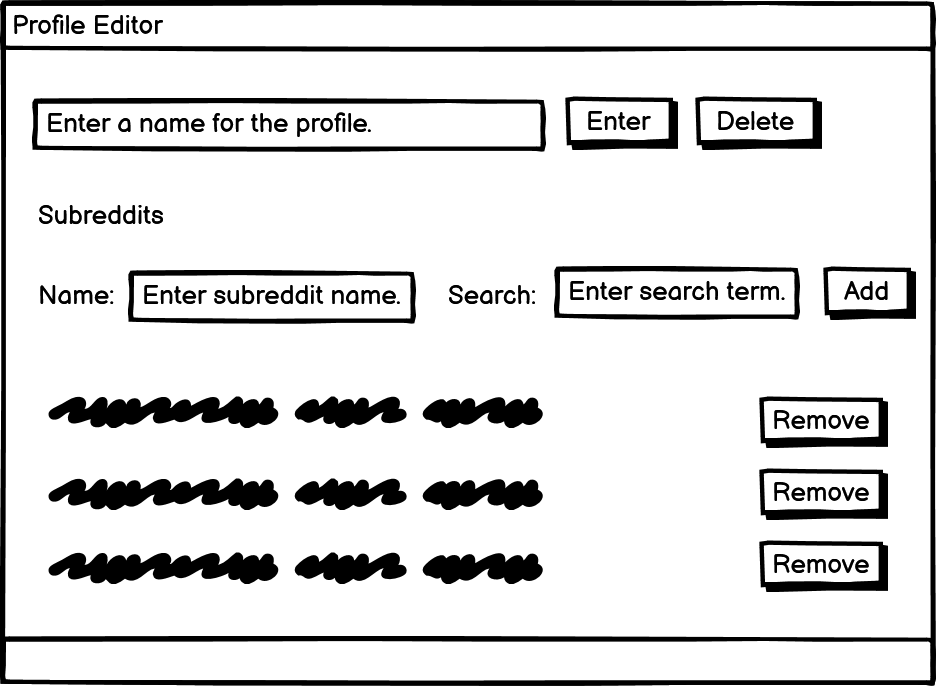
\includegraphics[width=0.5\textwidth]{figures/wireframe-profile-editor.png}
    \caption{Wire-frame of the proposed profile editor GUI.}
\end{figure}

Finally, the settings window should be easily navigable and contain various settings for functionality and visuals of the application. The different types of settings will be separated into tabs, and each setting will have its own row in the tab it belongs to.

\begin{figure}[h]
    \centering
    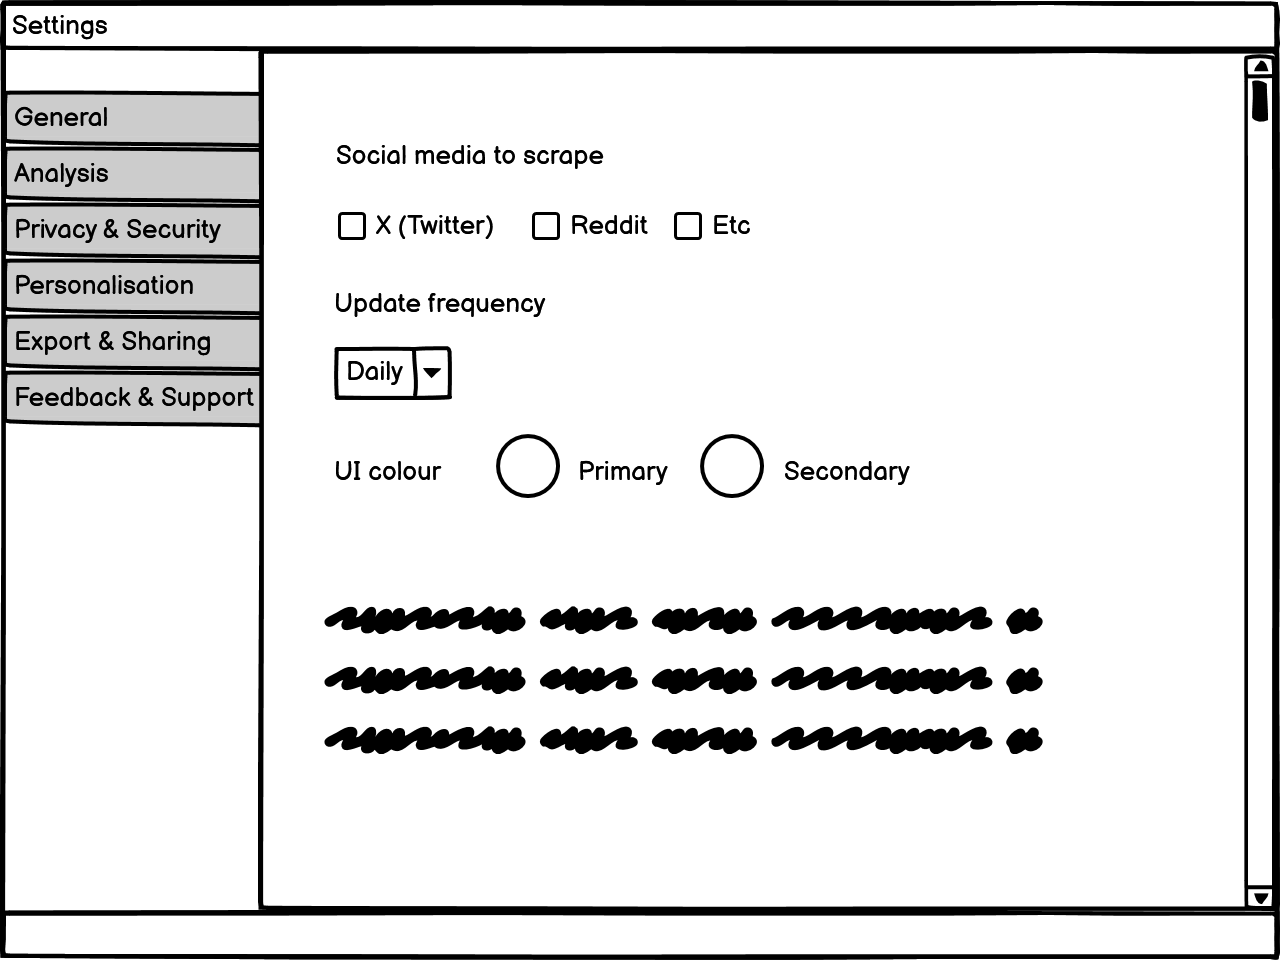
\includegraphics[width=0.7\textwidth]{figures/wireframe-settings.png}
    \caption{Wire-frame of the proposed settings GUI.}
\end{figure}

\section{Model Selection}
When selecting the model to use for this project, it was important to consider model performance, versatility, and the ability to handle complex linguistic patterns. While alternative models such as LSTM, Single CNN with FastText, and 2-L CNN with GRU have shown to be effective with NLP tasks, BERT was chosen as the preferred choice for several reasons.

    \subsection{Contextual Understanding}
    BERT's bidirectional architecture allows it to capture context information from preceding and succeeding words within the text, this addresses the complexities of language and sentiment expression highlighted by \citet{nasukawa2003sentiment, d2019sentiment}. Unlike LSTM, which processes text sequentially, BERT's bidirectional, contextual approach allows it to capture nuances and ambiguities in sentiment, making it perfect for the long-form posts prevalent in this task.

    \subsection{Pre-trained Language Representation}
    BERT is able to generalise well across diverse sentiment analysis tasks due to its pre-trained representation offering rich understanding of language semantics \citep{dhola2021comparative, rangila2022sentiment}. It's pre-trained knowledge reduces the need for extensive fine-tuning, facilitating transfer learning and aligning with \citet{malic2019social}'s recommendation of systematic data collection and storage.

    \subsection{Transformers Architecture}
    The transformer architecture allows for parallel processing and hence efficient training on large-scale datasets \citep{kansara2020comparison}. BERT's architecture and self-attention mechanism lets BERT capture long-range dependencies in long-form text, which overcomes issues with data sparsity and polarity shift often seen with traditional models \citep{abirami2017survey, kamruzzaman2021comparative}.

    \subsection{Transfer Learning}
    Due to its transfer learning capabilities, BERT is adaptable to diverse sentiment tasks with minimal labelled data, which aligns with the need in market research for innovative approaches that provide high value information \citep{vikram2020use, gerdes2008integrative}. By fine-tuning BERT on task-specific datasets, its pre-trained knowledge can be harnessed to achieve high performance in sentiment analysis.

    \subsection{Polysemy and Ambiguity Handling}
    BERT's bidirectional context modeling allows it to disambiguate polysemous words and resolve ambiguities based on surrounding context \citep{zhou2016linguistic}. This is particularly useful for analysing social media posts, where sentiment can vary based on the broader discourse and user engagement such as favourites and comments \citep{mostafa2013more, lange2011people}.

\section{Development Methodology}
For the development of this tool, an Agile-inspired approach will be used and adapted to a single-person development team. This will allow for iterative development, allowing for flexibility and adaptability throughout the process. The development process will be divided into five key phases which each focus on a specific aspect of the application:

\begin{itemize}
    \item \textbf{Sentiment Analysis Model}: This phase will encompass the training, fine-tuning, and prediction functionality of the chosen models.
    \item \textbf{Social Media Data Collection}: This phase will focus on collecting data from social media platforms for analysis. All interactions with social media APIs will be implemented in this phase.
    \item \textbf{Database Management}: With the data collection implemented, the focus will shift to setting up and managing the storage of collected and analysed data, and implementing secure encryption techniques.
    \item \textbf{Data Visualisation}: Once the analysed data is stored, the next phase will involve processing the data and visualising it in various charts, such as a line graph showing sentiment over time.
    \item \textbf{Graphical User Interface}: The final phase of development will revolve around designing and implementing a GUI for the application. The GUI will be built to be intuitive and linked to the previously created functionality.
\end{itemize}

Through each stage of development, an iterative approach will be taken. The work will be broken down into smaller, more manageable tasks, such as the creation of classes and implementation of specific functions, these tasks will be prioritised based on importance and dependencies, and completed in short iterations or `sprints'. To facilitate this, the code will be split into many modules and objects, each with distinct functions to allow for code reusability.

Continuous Integration (CI) practices will be implemented, after each iteration the code will be tested through unit tests and integration tests to validate the interactions between different modules and functions. The codebase will then be pushed to a GitHub repository to allow for version control.

The code will be well documented through comments and type-hinting, ensuring clarity and consistency in the codebase, and allowing knowledge of the application's inner workings to be accessible should any other people add to the development in the future.

This Agile-inspired approach will facilitate flexibility and adaptability, allowing effective response to requirement and priority changes.

\section{Testing Strategy}
In order to ensure accuracy, reliability, and usability, the sentiment analysis tool must implement effective testing strategies. The primary objectives of these strategies include verifying the precision of sentiment analysis results, validating the functionality of the application components, and assessing the overall user experience provided by the GUI. To achieve this, various types of testing will be used:

\begin{itemize}
    \item \textbf{Unit Testing}: the process of asserting the functionality of small, individual units or components of the application in isolation. It ensures that each component works as expected and verifies the functional integrity of the sentiment analysis tool.
    \item \textbf{Integration Testing}: focuses on validating interactions between different modules and components within the application. It tests the communication among all parts of the application, including data collection, database management, sentiment analysis algorithms, and the GUI functionality.
    \item \textbf{System Testing}: an evaluation of the sentiment analysis tool as a whole, assessing its compliance with the requirements and user expectations. This tests the end-to-end functionality of the application, encompassing all of its components and functions.
    \item \textbf{User Acceptance Testing}: the process of end-users assessing the usability, functionality, and overall user experience of the sentiment analysis tool. This makes sure that the application meets the needs and expectations of its intended users.
\end{itemize}